\section{Addestramento su dataset filtrato}

\subsection{Addestramento dei modelli}

L'addestramento dei tre modelli è stato effettuato tramite uno script Python che impiega la libreria di Ultralytics per caricare ed addestrare il modello:

\begin{figure}[ht]
    \centering
    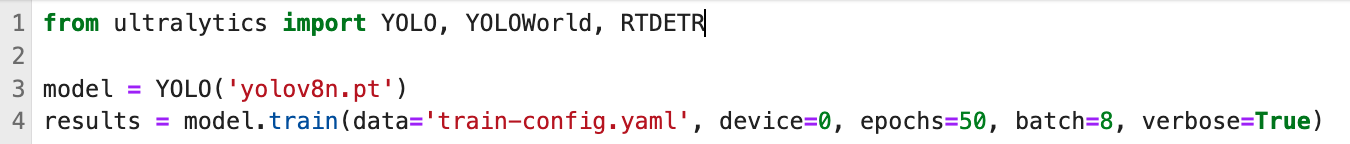
\includegraphics[width=1\textwidth]{files/capitoli/4-sperimentazione-risultati/assets/train-script.png}
    \caption{\label{fig:train-script}Script per l'addestramento di 'yolov8n'}
\end{figure}

\subsubsection{Parametri}
Il metodo \texttt{train}\cite{43} dei modelli di Ultralytics permette di configurare una vasta varietà di parametri, quelli di nostro interesse sono:
\begin{itemize}
    \item \textbf{data}: path al file di configurazione del dataset, in cui vengono specificati il path dei dati e le classi su cui addestrare il modello. In questo caso \texttt{train-config.yaml} indica i path ai subset train e val
    \item \textbf{device}: specifica il dispositivo/i computazionali per l'addestramento
    \item \textbf{epochs}: numero totale delle epochs di addestramento. Ciascuna epoch rappresenta un passaggio completo sull'intero dataset, perciò modificare questo valore influenza la durata dell'addestramento e le prestazioni del modello.
    \item \textbf{batch}: numero di campioni di addestramento processati simultaneamente durante ogni iterazione. Aumentare il batch size può migliorare l'efficienza computazionale, ma richiede più memoria.
    \item \textbf{verbose}: abilita un output dettagliato durante l'addestramento, fornendo log dettagliati e aggiornamenti sul progresso
\end{itemize}

\subsubsection{Augmentations}
Il metodo \texttt{train} di ultralytics implementa internamente delle tecniche di augmentation, essenziali per migliorare la robustezza e le prestazioni dei modelli YOLO. Durante l'addestramento vengono quindi eseguite le seguenti tecniche:

\begin{itemize}
    \item Adjustment of Hue
    \item Adjustment of Saturation
    \item Adjustment of Brightness
    \item Translation
    \item Scaling
    \item Horizontal Flipping
    \item Mixup
    \item Cutout
    \item Crop
\end{itemize}

\newpage

\subsection{Test dei modelli addestrati sul dataset filtrato}
Il primo addestramento dei modelli è stato condotto sul dataset \texttt{filtered-data} per un totale di 50 epochs, in modo da ottenere un buon equilibrio tra velocità di addestramento e capacità del modello; il batch size è stato impostato ad 8 per evitare problemi di memoria sui dispositivi.

Dopo aver completato l'addestramento, ho testato i modelli utilizzando il metodo \texttt{val} sulla migliore configurazione dei parametri interni ottenuta durante le 50 epochs di addestramento, ottenendo i seguenti risultati:

\begin{figure}[ht]
    \centering
    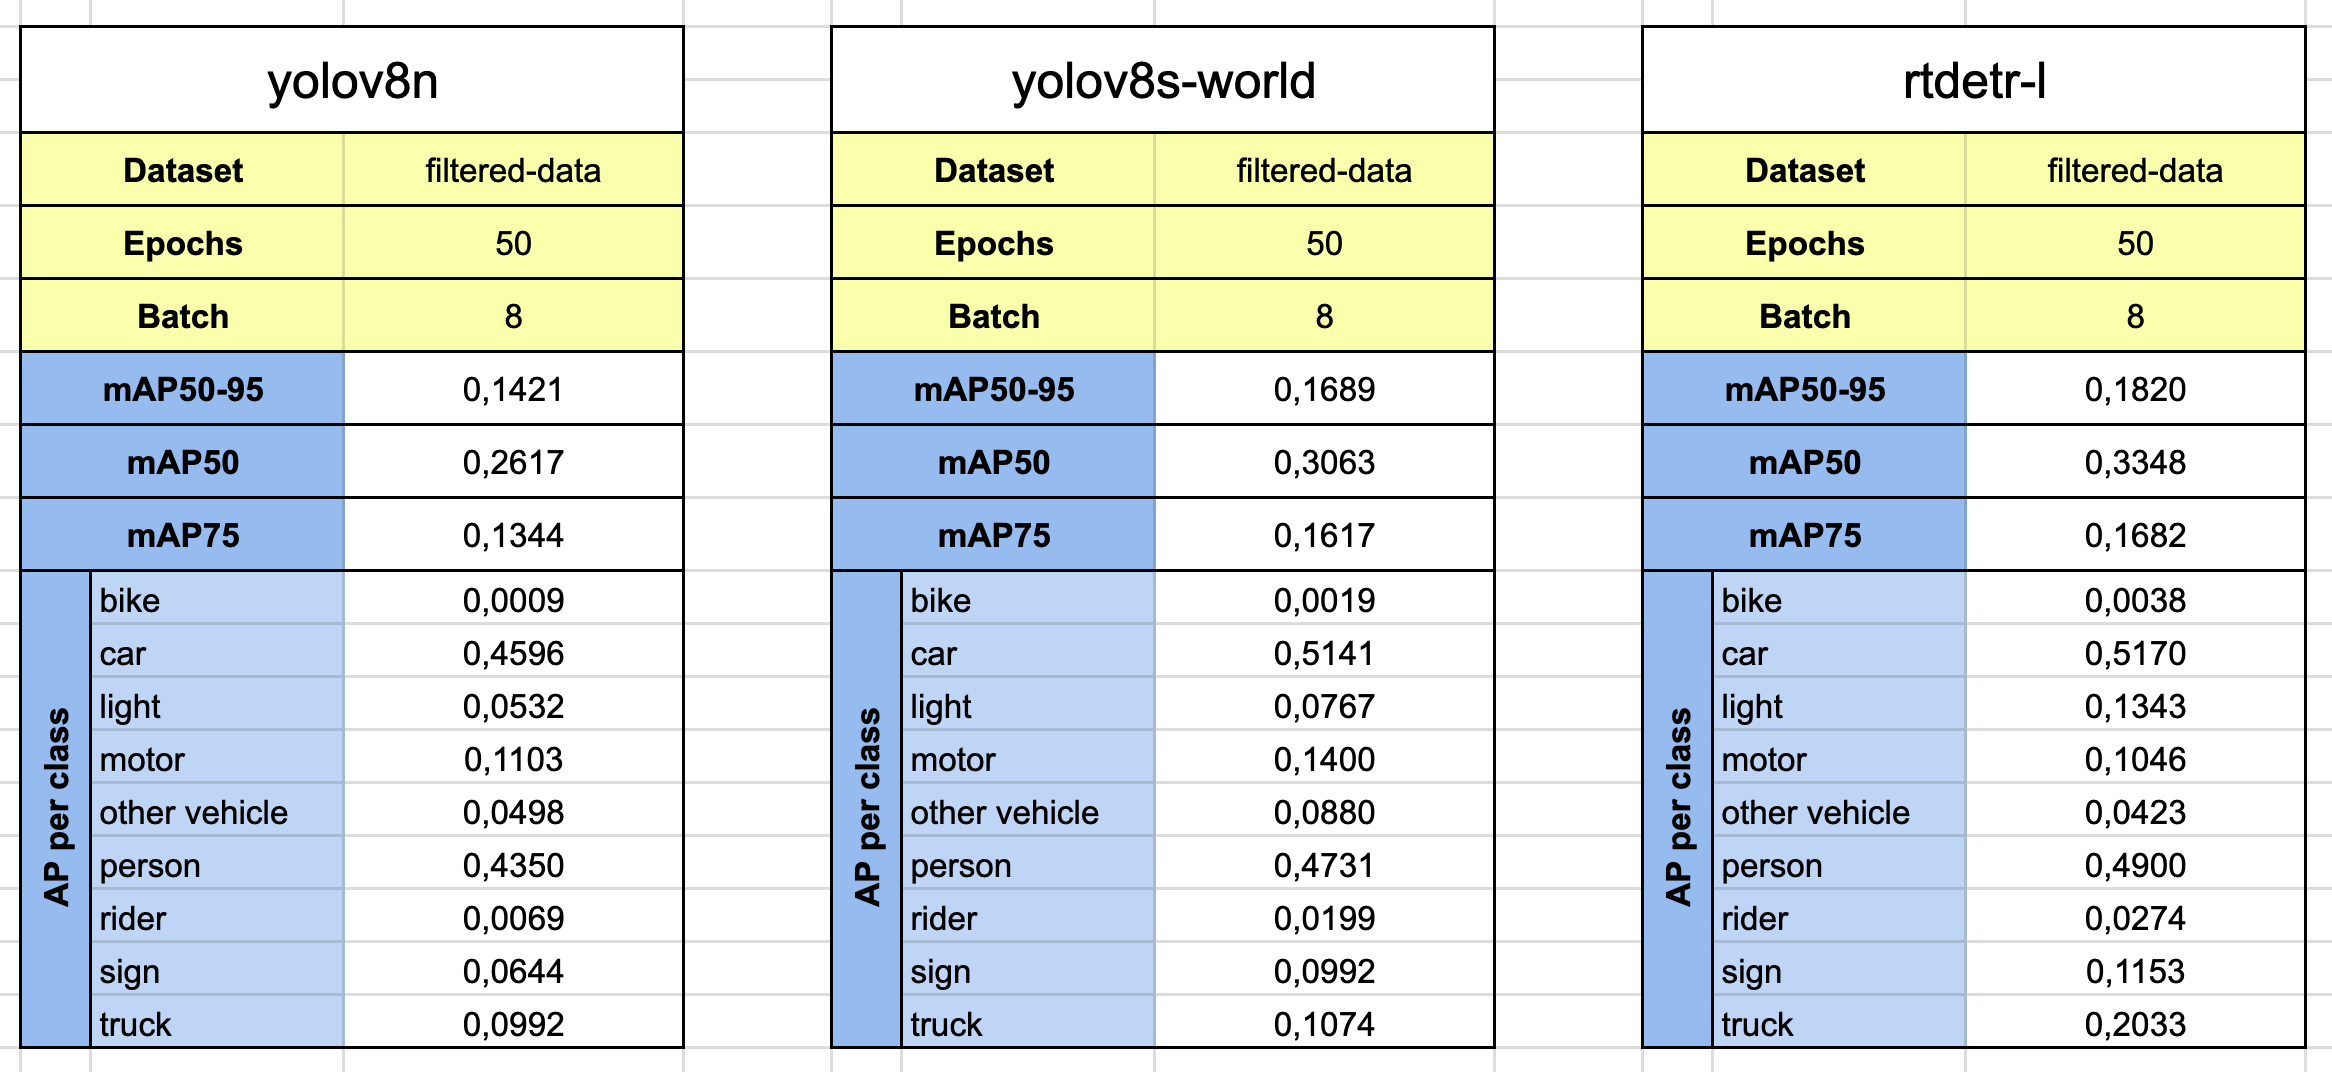
\includegraphics[width=1\textwidth]{files/capitoli/4-sperimentazione-risultati/assets/filtered-data-metrics.png}
    \caption{\label{fig:filtered-data-metrics}Risultati test dei modelli addestrati sul dataset filtrato}
\end{figure}

Possiamo osservare un notevole miglioramento delle prestazioni rispetto ai test precedenti dei modelli, già con questo primo addestramento effettuato su \texttt{filtered-data}.
Questo dimostra come il fine-tuning sia essenziale per ottimizzare i modelli su tipologie di dati specifiche come le nostre immagini termiche.

\clearpage

\begin{figure}[ht]
    \centering
    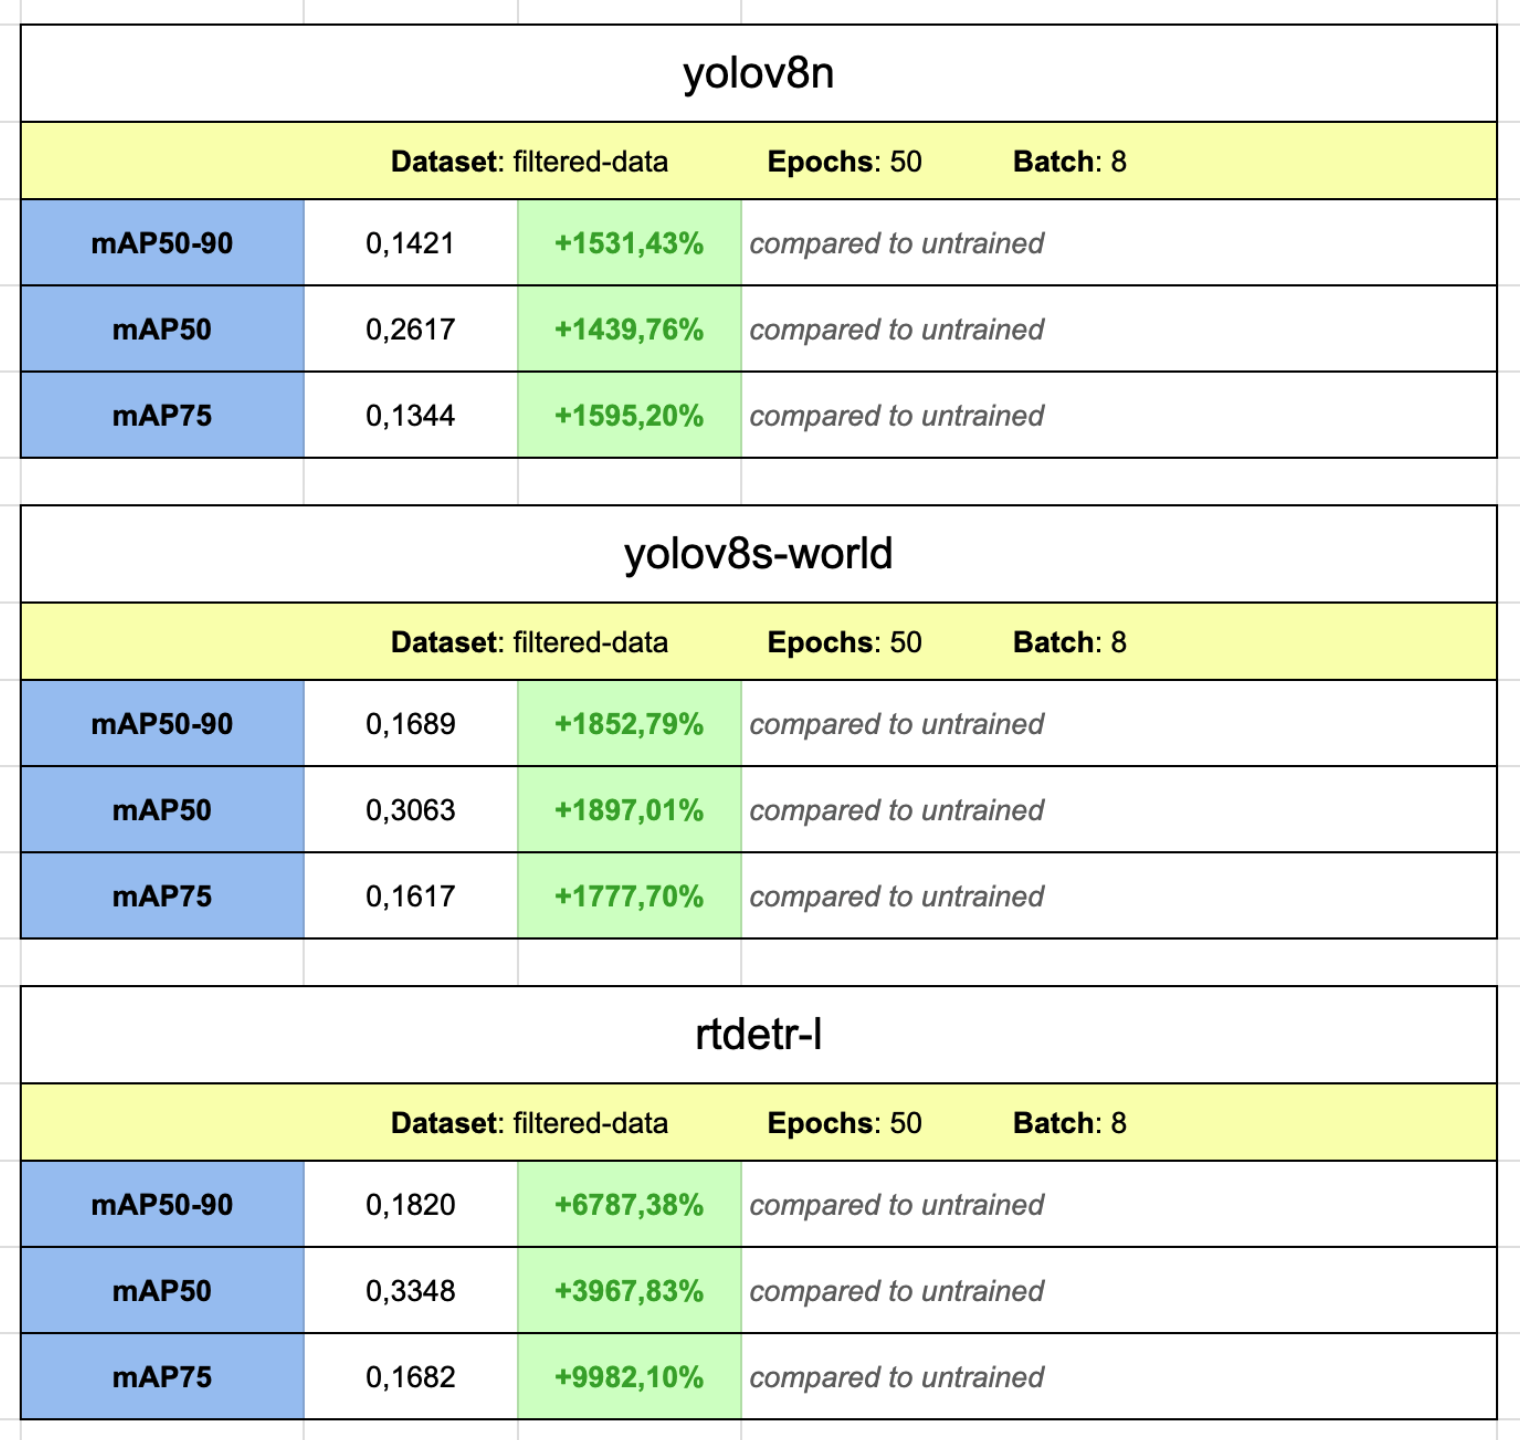
\includegraphics[width=0.9\textwidth]{files/capitoli/4-sperimentazione-risultati/assets/filtered-data-compare.png}
    \caption{\label{fig:filtered-data-compare}Confronto tra i risultati dei test dei modelli addestrati sul dataset filtrato e quelli dei precedenti test}
\end{figure}

\clearpage

\begin{figure}[ht]
    \centering
    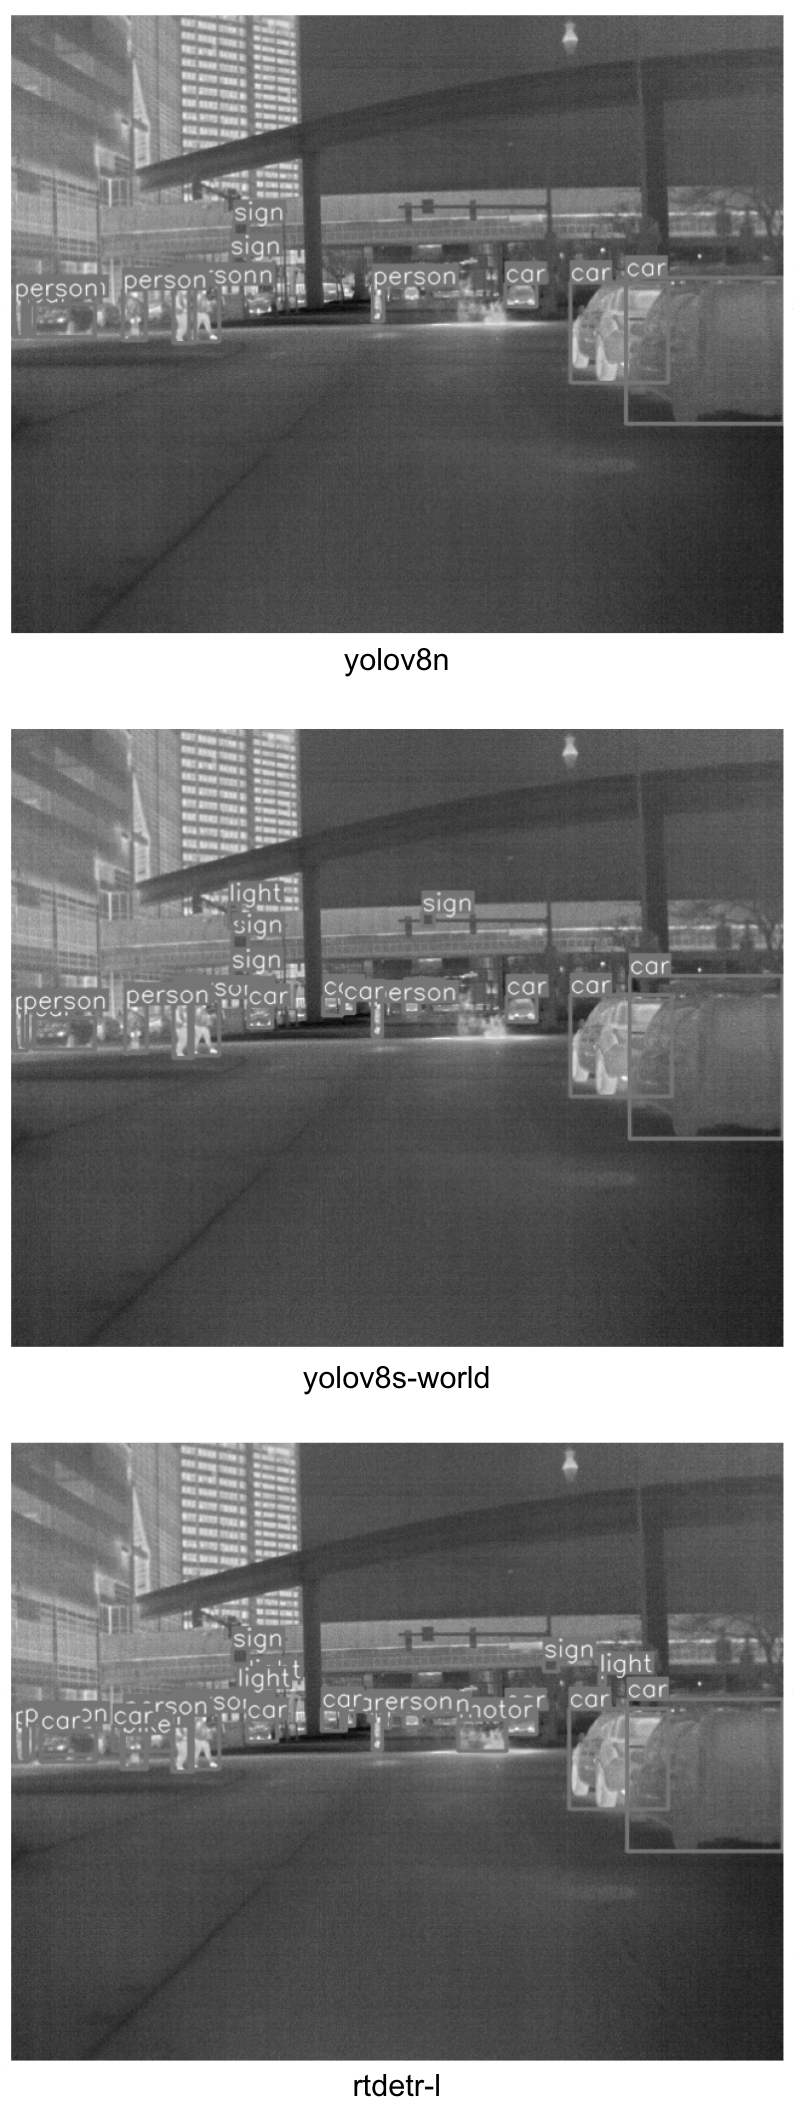
\includegraphics[width=0.6\textwidth]{files/capitoli/4-sperimentazione-risultati/assets/filtered-data-detections.png}
    \caption{\label{fig:initial-detections}Detections effettutate dai modelli addestrati sul dataset filtrato}
\end{figure}

\clearpage